\hypertarget{resampling}{%
\chapter{Resampling}\label{resampling}}

This chapter introduces \textbf{resampling methods}, which are used to
quantify the precision of an estimate. As examples, we'll use results a
vaccine trial to estimate the efficacy of the vaccine, data from the
Behavioral Risk Factor Surveillance System to estimate the average
height of men in the U.S., and data from the General Social Survey to
see how support for gun control has changed over time.

\hypertarget{vaccine-testing}{%
\section{Vaccine Testing}\label{vaccine-testing}}

Suppose you read a report about a new vaccine and the manufacturer says
it is 67\% effective at preventing disease. You might wonder where that
number comes from, what it means, and how confident we should be that it
is correct.

Results like this often come from a randomized controlled trial(RCT),
which works like this:

\begin{itemize}
\item
  You recruit a large group of volunteers and divide them into two
  groups at random: the ``treatment group'' receives the vaccine; the
  ``control group'' does not.
\item
  Then you follow both groups for a period of time and record the number
  of people in each group who are diagnosed with the disease.
\end{itemize}

As an example, suppose you recruit 43,783 participants and they are
assigned to groups with approximately the same size.

\begin{lstlisting}[language=Python]
n_control = 21885
n_treatment = 21911
\end{lstlisting}

During the observation period, 468 people are diagnosed with the
disease: 352 in the control group and 116 in the treatment group.

\begin{lstlisting}[language=Python]
k_control = 352
k_treatment = 116
\end{lstlisting}

We can use these results to compute the risk of getting the disease for
each group, in cases per 1000 people

\begin{lstlisting}[language=Python]
risk_control = k_control / n_control * 1000
risk_control
\end{lstlisting}

\begin{lstlisting}[]
16.084075851039522
\end{lstlisting}

\begin{lstlisting}[language=Python]
risk_treatment = k_treatment / n_treatment * 1000
risk_treatment
\end{lstlisting}

\begin{lstlisting}[]
5.294144493633334
\end{lstlisting}

The risk is substantially lower in the treatment group -- about 5 per
1000, compared to 16 -- which suggests that the vaccine is effective. We
can summarize these results by computing relative risk, which is the
ratio of the two risks (see
\url{https://en.wikipedia.org/wiki/Relative_risk}):

\begin{lstlisting}[language=Python]
relative_risk = risk_treatment / risk_control
relative_risk
\end{lstlisting}

\begin{lstlisting}[]
0.3291544097817203
\end{lstlisting}

The relative risk in this example is about 0.33, which means that the
risk of disease in the treatment group is 33\% of the risk in the
control group. Equivalently, we could report the complement of relative
risk, which is \textbf{efficacy}:

\begin{lstlisting}[language=Python]
efficacy = 1 - relative_risk
efficacy
\end{lstlisting}

\begin{lstlisting}[]
0.6708455902182797
\end{lstlisting}

In this example the efficacy is \passthrough{\lstinline!0.67!}, which
means that the vaccine reduces the risk of disease by 67\%. That's good
news, but as skeptical data scientists, we should not assume that it is
perfectly accurate. There are any number of things that might have gone
wrong.

For example, if people in the treatment group know they have been
vaccinated, they might take fewer precautions to prevent disease, and
people in the control group might be more careful. That would affect the
estimated efficacy, which is why a lot of trials are ``blinded'',
meaning that the subjects don't know which group they are in.

The estimate would also be less accurate if people in either group don't
follow the protocol. For example, someone in the treatment group might
not complete treatment, or someone in the control group might receive
treatment from another source.

And there are many other possible sources of error, including honest
mistakes and deliberate fraud.

In general it is hard to know whether estimates like this are accurate;
nevertheless, there are things we can do to assess their quality.

When estimates are reported in scientific journals, they almost always
include one of two measurements of uncertainty: a standard error or a
confidence interval. In the next section, I'll explain what they mean
and show how to compute them.

\hypertarget{simulating-one-group}{%
\section{Simulating One Group}\label{simulating-one-group}}

In our hypothetical example, there are 21 911 people in the treatment
group and 116 of them got the disease, so the estimated risk is about 5
cases per 1000 people.

\begin{lstlisting}[language=Python]
n_treatment, k_treatment, risk_treatment
\end{lstlisting}

\begin{lstlisting}[]
(21911, 116, 5.294144493633334)
\end{lstlisting}

But it's easy to imagine that there might have been a few more cases, or
fewer, just by chance. For example, if there had been 10 more cases, the
estimated risk would be 5.8 per 1000, and if there had been 10 fewer, it
would be 4.8.

\begin{lstlisting}[language=Python]
126 / n_treatment * 1000, 106 / n_treatment * 1000
\end{lstlisting}

\begin{lstlisting}[]
(5.750536260325863, 4.837752726940806)
\end{lstlisting}

That's a big enough difference that we should wonder how much
variability there is in the estimate due to random variation. We'll
answer that question in three steps:

\begin{itemize}
\item
  We'll write a function that uses a random number generator to simulate
  the trial.
\item
  Then we'll run the function 1000 times to see how much the estimate
  varies.
\item
  And we'll summarize the results.
\end{itemize}

The following function takes two parameters: \passthrough{\lstinline!n!}
is the number of people in the group (treatment or control) and
\passthrough{\lstinline!p!} is the probability that any of them gets the
disease.

\begin{lstlisting}[language=Python]
import numpy as np

def simulate_group(n, p):
    xs = np.random.random(size=n)
    k = np.sum(xs < p)
    return k / n * 1000
\end{lstlisting}

The first line generates an array of \passthrough{\lstinline!n!} random
values between 0 and 1. The values are distributed uniformly in this
range, so the probability that each one is less than
\passthrough{\lstinline!p!} is\ldots{} \passthrough{\lstinline!p!}.

The second line counts how many of the values are less than
\passthrough{\lstinline!p!}, that is, how many people in the simulated
group get the disease. Then the function returns the estimated risk.

Here's how we call this function, passing as arguments the size of the
treatment group and the estimated risk:

\begin{lstlisting}[language=Python]
p = k_treatment / n_treatment
simulate_group(n_treatment, p)
\end{lstlisting}

\begin{lstlisting}[]
6.070010497010633
\end{lstlisting}

The result is the estimated risk from a simulated trial. If we run this
function 1000 times, it's like running the trial over and over.

\begin{lstlisting}[language=Python]
t = [simulate_group(n_treatment, p)
     for i in range(1000)]
\end{lstlisting}

The result is a list of estimated risks that shows how much we expect
the results of the trial to vary due to randomness. We can use a KDE
plot to visualize the distribution of these estimates.

\begin{lstlisting}[language=Python]
import matplotlib.pyplot as plt
import seaborn as sns

sns.kdeplot(t, label='control')

plt.xlabel('Risk of disease (cases per 1000)')
plt.ylabel('Probability density')
plt.title('Estimated Risks from Simulation');
\end{lstlisting}

\begin{center}
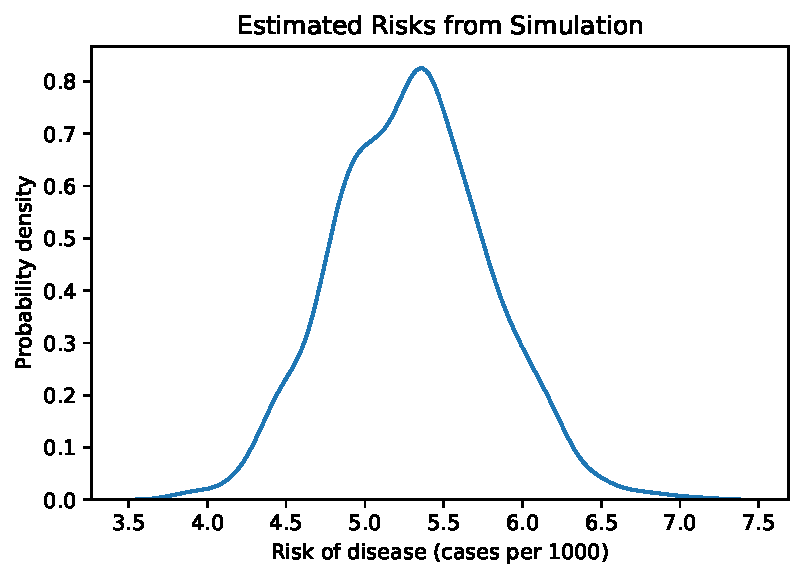
\includegraphics[scale=0.75]{chapters/11_resampling_files/11_resampling_30_0.pdf}
\end{center}

The mean of this distribution is about 5.3, which is close to the
observed risk, as we should expect.

\begin{lstlisting}[language=Python]
np.mean(t), risk_treatment
\end{lstlisting}

\begin{lstlisting}[]
(5.299210442243623, 5.294144493633334)
\end{lstlisting}

The width of this distribution indicates how much variation there is in
the estimate due to randomness. One way to quantify the width of the
distribution is the standard deviation.

\begin{lstlisting}[language=Python]
standard_error = np.std(t)
standard_error
\end{lstlisting}

\begin{lstlisting}[]
0.48944411243624414
\end{lstlisting}

This result is called the \textbf{standard error} (see
\url{https://en.wikipedia.org/wiki/Standard_error}).

Another way to quantify the width of the distribution is an interval
between two percentiles. For example, if we compute the 5th and 95th
percentiles, the interval we get contains 90\% of the simulated
estimates.

\begin{lstlisting}[language=Python]
confidence_interval = np.percentile(t, [5, 95])
confidence_interval
\end{lstlisting}

\begin{lstlisting}[]
array([4.47263931, 6.11793163])
\end{lstlisting}

This result is called a \textbf{confidence interval} ; specifically,
this one is a ``90\% confidence interval'', or 90\% CI (see
\url{https://en.wikipedia.org/wiki/Confidence_interval}). If we assume
that the observed risk is correct, and we run the same trial many times,
we expect 90\% of the estimates to fall in this interval.

Standard errors and confidence intervals quantify our uncertainty about
the estimate due to random variation from one trial to another.

\hypertarget{simulating-the-trial}{%
\section{Simulating the Trial}\label{simulating-the-trial}}

If that's not making sense yet, let's try another example. In the
previous section we simulated one group and estimated their risk. Now
we'll simulate both groups and estimate the efficacy of the vaccine.

The following function takes as parameters the size of the two groups
and their actual risks.

\begin{lstlisting}[language=Python]
def simulate_trial(n1, p1, n2, p2):
    risk1 = simulate_group(n1, p1)
    risk2 = simulate_group(n2, p2)
    efficacy = 1 - risk2 / risk1
    return efficacy
\end{lstlisting}

If we call this function once, it simulates both groups, computes their
risks in each group, and uses the results to estimate the efficacy of
the treatment (assuming that the first group is the control).

\begin{lstlisting}[language=Python]
p1 = k_control / n_control
p2 = k_treatment / n_treatment
simulate_trial(n_control, p1, n_treatment, p2)
\end{lstlisting}

\begin{lstlisting}[]
0.6891301291299345
\end{lstlisting}

If we call it 1000 times, the result is a list of estimated efficacies
from 1000 simulated trials.

\begin{lstlisting}[language=Python]
t2 = [simulate_trial(n_control, p1, n_treatment, p2)
      for i in range(1000)]
\end{lstlisting}

We can use a KDE plot to visualize the distribution of these estimates.

\begin{lstlisting}[language=Python]
sns.kdeplot(t2)

plt.xlabel('Efficacy')
plt.ylabel('Probability density')
plt.title('Estimated Efficacy from Simulation');
\end{lstlisting}

\begin{center}
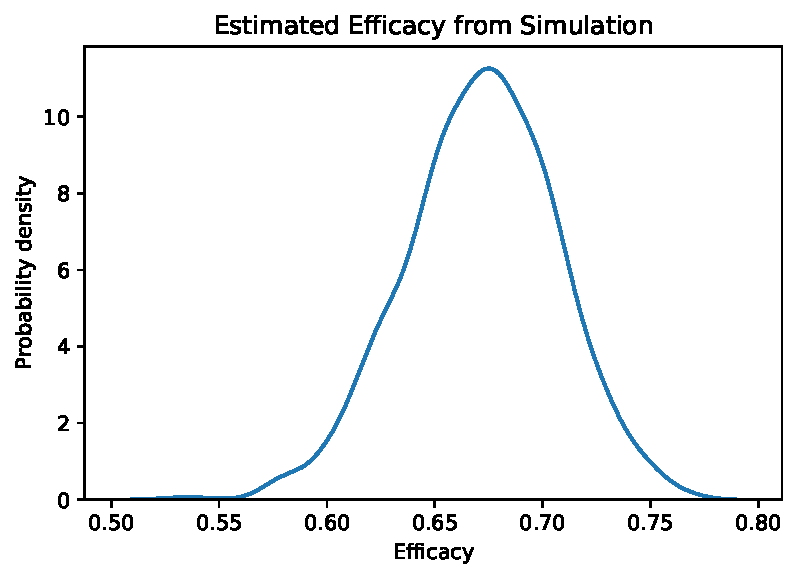
\includegraphics[scale=0.75]{chapters/11_resampling_files/11_resampling_45_0.pdf}
\end{center}

The mean of this distribution is close to the efficacy we computed with
the results of the actual trial.

\begin{lstlisting}[language=Python]
np.mean(t2), efficacy
\end{lstlisting}

\begin{lstlisting}[]
(0.6713727268668117, 0.6708455902182797)
\end{lstlisting}

The standard deviation of this distribution is the standard error of the
estimate.

\begin{lstlisting}[language=Python]
np.std(t2)
\end{lstlisting}

\begin{lstlisting}[]
0.035068503707114076
\end{lstlisting}

In a scientific paper, we could report the estimated efficacy and
standard error as 0.67 (SE 0.035). As an alternative, we can use
percentiles to compute a 90\% confidence interval.

\begin{lstlisting}[language=Python]
np.percentile(t2, [5, 95])
\end{lstlisting}

\begin{lstlisting}[]
array([0.61344412, 0.72785182])
\end{lstlisting}

In a scientific paper, we could report these results as 0.67, 90\% CI
{[}0.61, 0.72{]}".

The standard error and confidence interval represent nearly the same
information. In general, I prefer to report a confidence interval
because it is easier to interpret.

\begin{itemize}
\item
  Formally, it means that if we run the same experiment again, we expect
  90\% of the results to fall between 61\% and 72\% (assuming that the
  estimated risks are correct).
\item
  More casually, it means that it is plausible that the actually
  efficacy is as low as 61\%, or as high as 72\% (assuming there are no
  sources of error other than random variation).
\end{itemize}

\hypertarget{estimating-means}{%
\section{Estimating Means}\label{estimating-means}}

In the previous examples, we've estimated risk, which is a proportion,
and efficacy, which is a ratio of two proportions. As a third example,
let's estimate a mean.

Suppose we want to estimate the average height of men in the United
States. It would be impractical to measure everyone in the country, but
if we choose a random sample of the population and measure the people in
the sample, we can use the mean of the measurements to estimate the mean
of the population.

Ideally, the sample should be \textbf{representative}, which means that
everyone in the population has an equal chance of appearing in the
sample. In general, that's not easy to do. Depending on how you recruit
people, your sample might have too many tall people or too many short
people.

But let's suppose we have a representative sample of 103 adult male
residents of the United States, the average height in the sample is 177
cm, and the standard deviation is 8.4 cm.

If someone asks for your best guess about the height of mean in the
U.S., you would report 177 cm. But how accurate do you think this
estimate is? If you only measure 103 people from a population of about
100 million adult males, it seems like the actual average in the
population might be substantially higher or lower.

Again, we can use random simulation to quantify the uncertainty of this
estimate. As we did in the previous examples, we will assume for
purposes of simulation that the estimates are correct, and simulate the
sampling process 1000 times.

The following function takes as parameters the size of the sample,
\passthrough{\lstinline!n!}, the presumed average height in the
population, \passthrough{\lstinline!mu!}, and the presumed standard
deviation, \passthrough{\lstinline!std!}.

\begin{lstlisting}[language=Python]
def simulate_sample_mean(n, mu, sigma):
    sample = np.random.normal(mu, sigma, size=n)
    return sample.mean()
\end{lstlisting}

This function generates \passthrough{\lstinline!n!} random values from a
normal distribution with the given mean and standard deviation, and
returns their mean.

We can run it like this, using the observed mean and standard deviation
from the sample as the presumed mean and standard deviation of the
population.

\begin{lstlisting}[language=Python]
n_height = 103
mean_height = 178
std_height = 7.97

simulate_sample_mean(n_height, mean_height, std_height)
\end{lstlisting}

\begin{lstlisting}[]
178.64931744931997
\end{lstlisting}

If we run it 1000 times, it simulates the sampling and measurement
process and returns a list of results from 1000 simulated experiments.

\begin{lstlisting}[language=Python]
t3 = [simulate_sample_mean(n_height, mean_height, std_height)
      for i in range(1000)]
\end{lstlisting}

We can use a KDE plot to visualize the distribution of these values.

\begin{lstlisting}[language=Python]
sns.kdeplot(t3)

plt.xlabel('Average height (cm)')
plt.ylabel('Probability density')
plt.title('Sampling Distribution of the Mean');
\end{lstlisting}

\begin{center}
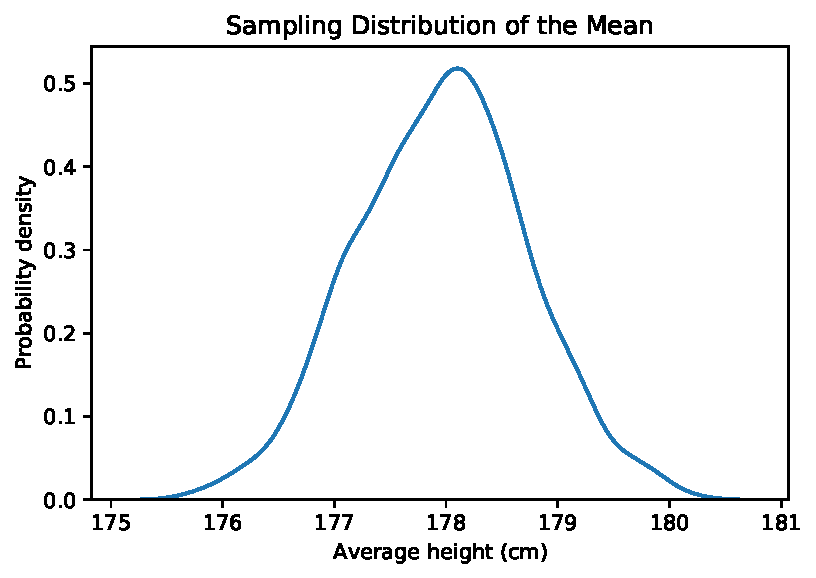
\includegraphics[scale=0.75]{chapters/11_resampling_files/11_resampling_60_0.pdf}
\end{center}

This distribution is called a \textbf{sampling distribution} because it
represents the variation in the results due to the random sampling
process. If we recruit 100 people and compute the mean of their heights,
the result might be as low as 175 cm, or as high as 179 cm, due to
chance.

The average of the sampling distribution is close to the presumed mean
of the population.

\begin{lstlisting}[language=Python]
np.mean(t3), mean_height
\end{lstlisting}

\begin{lstlisting}[]
(177.96271260304573, 178)
\end{lstlisting}

The standard deviation of the sampling distribution is the standard
error of the estimate.

\begin{lstlisting}[language=Python]
np.std(t3)
\end{lstlisting}

\begin{lstlisting}[]
0.7646185415617497
\end{lstlisting}

And we can use \passthrough{\lstinline!percentile!} to compute a 90\%
confidence interval.

\begin{lstlisting}[language=Python]
np.percentile(t3, [5, 95])
\end{lstlisting}

\begin{lstlisting}[]
array([176.7094124 , 179.22734483])
\end{lstlisting}

If I reported this result in a paper, I would say that the estimated
height of adult male residents of the U.S. is 177 cm, 90\% CI {[}176,
178{]} cm.

Informally, that means that the estimate could plausibly be off by about
a centimeter either way, just due to random sampling. But we should
remember that there are other possible sources of error, so we might be
off by more than that.

The confidence interval puts an upper bound on the precision of the
estimate; in this example, the precision of the estimate is 1 cm at
best, and might worse.

\hypertarget{the-resampling-framework}{%
\section{The Resampling Framework}\label{the-resampling-framework}}

The examples we've done so far fit into the framework shown in this
diagram:

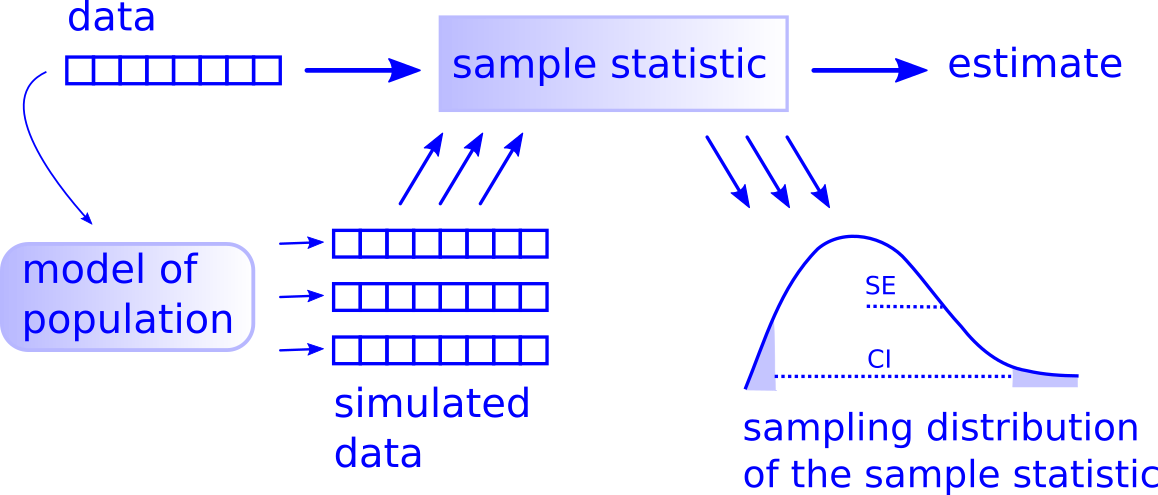
\includegraphics{figs/resampling.png}

Using data from an experiment, we compute a sample statistic. In the
vaccine example, we computed risks for each group and efficacy. In the
height example, we computed the average height in the sample.

Then we build a model of the sampling process. In the vaccine example,
the model assumes that everyone in each group has the same probability
of getting sick, and we use the data to choose the probability. In the
height example, the model assumes that heights are drawn from a normal
distribution, and we use the data to choose the parameters
\passthrough{\lstinline!mu!} and \passthrough{\lstinline!sigma!}.

We use the model to simulate the experiment many times. Each simulation
generates a dataset which we use to compute the sample statistic.

Finally, we collect the sample statistics from the simulations and use
them to plot the sampling distribution and compute standard errors and
confidence intervals.

I emphasize the role of the model in this framework because for a given
experiment there might be several possible models, each including some
elements of the real world and ignoring others.

For example, our model of the vaccine experiment assumes that everyone
in each group has the same risk, but that's probably not true. Here's
another version of \passthrough{\lstinline!simulate\_group!} that
includes variation in risk within each group.

\begin{lstlisting}[language=Python]
def simulate_variable_group(n, p):
    ps = np.random.uniform(0, 2*p, size=n)
    xs = np.random.random(size=n)
    k = np.sum(xs < ps)
    return k / n * 1000
\end{lstlisting}

This version of the function generates \passthrough{\lstinline!ps!},
which is an array of probabilities uniformly distributed between
\passthrough{\lstinline!0!} and \passthrough{\lstinline!2*n!}. Of
course, that's just a guess about how the probabilities might be
distributed in the group, but we can use it to get a sense of what
effect this distribution has on the results.

The rest of the function is the same a the previous version: it
generates \passthrough{\lstinline!xs!}, which is an array of random
values between \passthrough{\lstinline!0!} and
\passthrough{\lstinline!1!}. Then it compares
\passthrough{\lstinline!xs!} and \passthrough{\lstinline!ps!}, counting
the number of times \passthrough{\lstinline!p!} exceeds
\passthrough{\lstinline!x!}.

Here's how we call this function, simulating the treatment group.

\begin{lstlisting}[language=Python]
p = k_treatment / n_treatment
simulate_variable_group(n_treatment, p)
\end{lstlisting}

\begin{lstlisting}[]
5.339783670302587
\end{lstlisting}

The return value is the number of cases per 1000.

\textbf{Exercise:} Using this function to run 1000 simulations of the
treatment group. Compute the mean of the results and confirm that it is
close to the observed \passthrough{\lstinline!risk\_treatment!}. To
quantify the spread of the sampling distribution, compute the standard
error. How does it compare to the standard error we computed with the
original model, where everyone in the group has the same risk?

\textbf{Exercise:} The following is a version of
\passthrough{\lstinline!simulate\_trial!} that uses
\passthrough{\lstinline!simulate\_variable\_group!}, from the previous
exercise, to simulate the vaccine trial using the modified model, with
variation in risk within the groups.

Use this function to simulate 1000 trials. Compute the mean of the
sampling distribution and confirm that it is close to the observed
\passthrough{\lstinline!efficacy!}. Compute the standard error and
compare it to the standard error we computed for the original model.

\begin{lstlisting}[language=Python]
def simulate_variable_trial(n1, p1, n2, p2):
    risk1 = simulate_variable_group(n1, p1)
    risk2 = simulate_variable_group(n2, p2)
    efficacy = 1 - risk2 / risk1
    return efficacy
\end{lstlisting}

\textbf{Exercise:} One nice thing about the resampling framework is that
it is easy to compute the sampling distribution for other statistics.

For example, suppose we want to estimate the coefficient of variation
(standard deviation as a fraction of the mean) for adult male height.
Here's how we can compute it.

\begin{lstlisting}[language=Python]
cv = std_height / mean_height
cv
\end{lstlisting}

\begin{lstlisting}[]
0.044775280898876405
\end{lstlisting}

In this example, the standard deviation is about 5\% of the mean. The
following is a version of \passthrough{\lstinline!simulate\_sample!}
that generates a random sample of heights and returns the coefficient of
variation, rather than the mean.

\begin{lstlisting}[language=Python]
def simulate_sample_cv(n, mu, sigma):
    sample = np.random.normal(mu, sigma, size=n)
    return sample.std() / sample.mean()
\end{lstlisting}

Use this function to simulate 1000 samples with size
\passthrough{\lstinline!n=103!}, using
\passthrough{\lstinline!mean\_height!} for \passthrough{\lstinline!mu!}
and \passthrough{\lstinline!std\_height!} for
\passthrough{\lstinline!sigma!}. Plot the sampling distribution of the
coefficient of variation, and compute a 90\% confidence interval.

\hypertarget{gun-control}{%
\section{Gun Control}\label{gun-control}}

In Chapter 10 we used data from the General Social Survey, specifically
a variable called \passthrough{\lstinline!GUNLAW!}, to describe support
for a gun control law as a function of age, sex, and years of education.
Now let's come back to that dataset and see how the responses have
changed over time.

The following cell reloads the data.

\begin{lstlisting}[language=Python]
import pandas as pd

gss = pd.read_hdf('gss_eda.hdf', 'gss')
\end{lstlisting}

The column named \passthrough{\lstinline!GUNLAW!} records responses to
the question ``Would you favor or oppose a law which would require a
person to obtain a police permit before he or she could buy a gun?''

The response code \passthrough{\lstinline!1!} means yes;
\passthrough{\lstinline!2!} means no. It will be easier to work with
this variable if we recode it so \passthrough{\lstinline!0!} means no.

\begin{lstlisting}[language=Python]
gss['GUNLAW'].replace(2, 0, inplace=True)
gss['GUNLAW'].value_counts()
\end{lstlisting}

\begin{tabular}{lr}
\toprule
{} &  GUNLAW \\
\midrule
1.0 &   32038 \\
0.0 &    9975 \\
\bottomrule
\end{tabular}

For each year of the survey, I would like to compute the number of
respondents and the number who said they favor this law. I'll use
\passthrough{\lstinline!groupby!} to group the respondents by year of
interview and \passthrough{\lstinline!agg!} to compute two aggregation
functions, \passthrough{\lstinline!sum!} and
\passthrough{\lstinline!count!}.

\begin{lstlisting}[language=Python]
grouped = gss.groupby('YEAR')['GUNLAW']
agg = grouped.agg(['sum', 'count'])
agg.head()
\end{lstlisting}

\begin{tabular}{lrr}
\toprule
{} &     sum &  count \\
YEAR &         &        \\
\midrule
1972 &  1131.0 &   1562 \\
1973 &  1099.0 &   1470 \\
1974 &  1112.0 &   1459 \\
1975 &  1096.0 &   1450 \\
1976 &  1068.0 &   1472 \\
\bottomrule
\end{tabular}

The result is a \passthrough{\lstinline!DataFrame!} with two columns:
\passthrough{\lstinline!sum!} is the number of respondents who said
``yes''; \passthrough{\lstinline!count!} is the number of respondents
who were asked the question.

In some years the question was not asked, so I'll use
\passthrough{\lstinline!drop!} to remove those rows.

\begin{lstlisting}[language=Python]
zero = (agg['count'] == 0)
labels = agg.index[zero]
agg.drop(labels, inplace=True)
\end{lstlisting}

Now we can plot the percentage of respondents who favor gun control (at
least for this wording of the question) during each year.

\begin{lstlisting}[language=Python]
percent = agg['sum'] / agg['count'] * 100
percent.plot(style='o')

plt.xlabel('Year of survey')
plt.ylabel('Percent in favor')
plt.title('Support for gun control over time');
\end{lstlisting}

\begin{center}
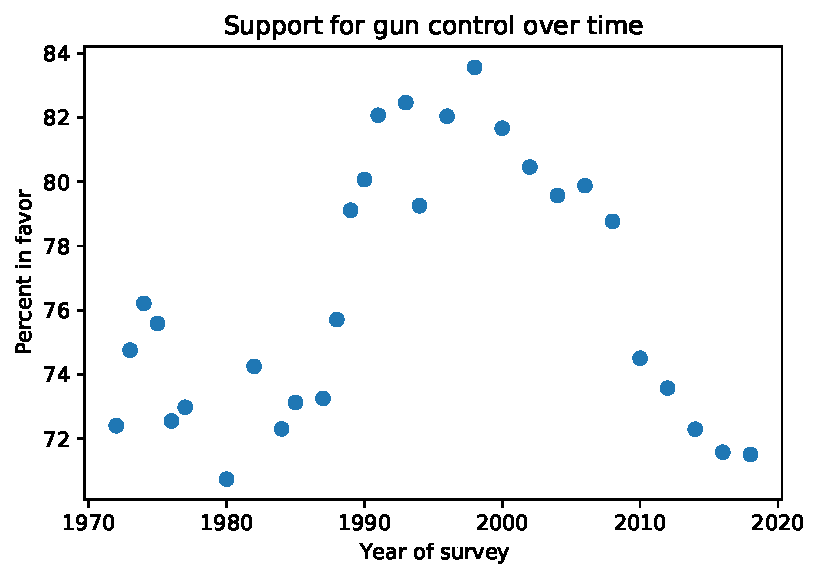
\includegraphics[scale=0.75]{chapters/11_resampling_files/11_resampling_94_0.pdf}
\end{center}

The results vary from year to year. It is hard to tell how much of this
variation is due to real changes in opinion, and how much is due to
random sampling. We can answer that question by computing confidence
intervals for each of these data points.

\textbf{Exercise:} Write a loop that goes through the rows in
\passthrough{\lstinline!agg!} and computes a confidence interval for
each year. You can use \passthrough{\lstinline!itertuples!} to iterate
the rows, like this:

\begin{lstlisting}[]
for year, k, n in agg.itertuples():
    print(year, k, n)
\end{lstlisting}

For each row, compute a 90\% confidence interval and plot it as a
vertical line. Then plot the data points and label the axes. The result
should give you a sense of how much variation we expect to see from year
to year due to random sampling.

You might want to use this version of
\passthrough{\lstinline!simulate\_group!}, which returns results as a
percentage, rather than per 1000.

\begin{lstlisting}[language=Python]
def simulate_group_percent(n, p):
    xs = np.random.random(size=n)
    k = np.sum(xs < p)
    return k / n * 100
\end{lstlisting}

\hypertarget{summary}{%
\section{Summary}\label{summary}}

Let's review the examples in this chapter:

\begin{enumerate}
\def\labelenumi{\arabic{enumi}.}
\item
  We started with results from a vaccine trial. We estimated the
  effectiveness of the vaccine and used simulation to draw a random
  sample from the sampling distribution of effectiveness. We used that
  sample to compute a standard error and a 90\% confidence interval,
  which measure the variability we would expect if we ran the experiment
  again (assuming that the observed efficacy is correct).
\item
  As a second example, we estimated the height of adult males in the
  U.S. and used simulation based on a normal model to compute the
  sampling distribution of the mean, standard error, and a confidence
  interval.
\item
  I presented the resampling framework, which shows what these examples
  have in common. We implemented a second model of the vaccine trial,
  based on the assumption that there is variation in risk within the
  treatment and control groups. The results from both models are
  similar, which suggests that the simple model is good enough for
  practical purposes.
\item
  One of the advantages of resampling, compared to mathematical
  analysis, is that it is easy to compute the sampling distribution of
  almost any statistic. As an exercise, you computed the sampling
  distribution of the coefficient of variation.
\item
  Finally, we used data from the General Social Survey to explore
  changes in support for gun control over time. We used resampling to
  compute and plot a confidence interval for the percentage of
  respondents in favor of a proposed law, for each year of the survey.
\end{enumerate}

The next chapter presents bootstrap sampling, which is a kind of
resampling particularly well suited for the kind of survey data we've
been working with.

